% !TeX spellcheck = en_GB
\begin{figure}[t!]
	\centering
	%%%%%% 20/12
	\begin{subfigure}[b]{0.49\textwidth}
		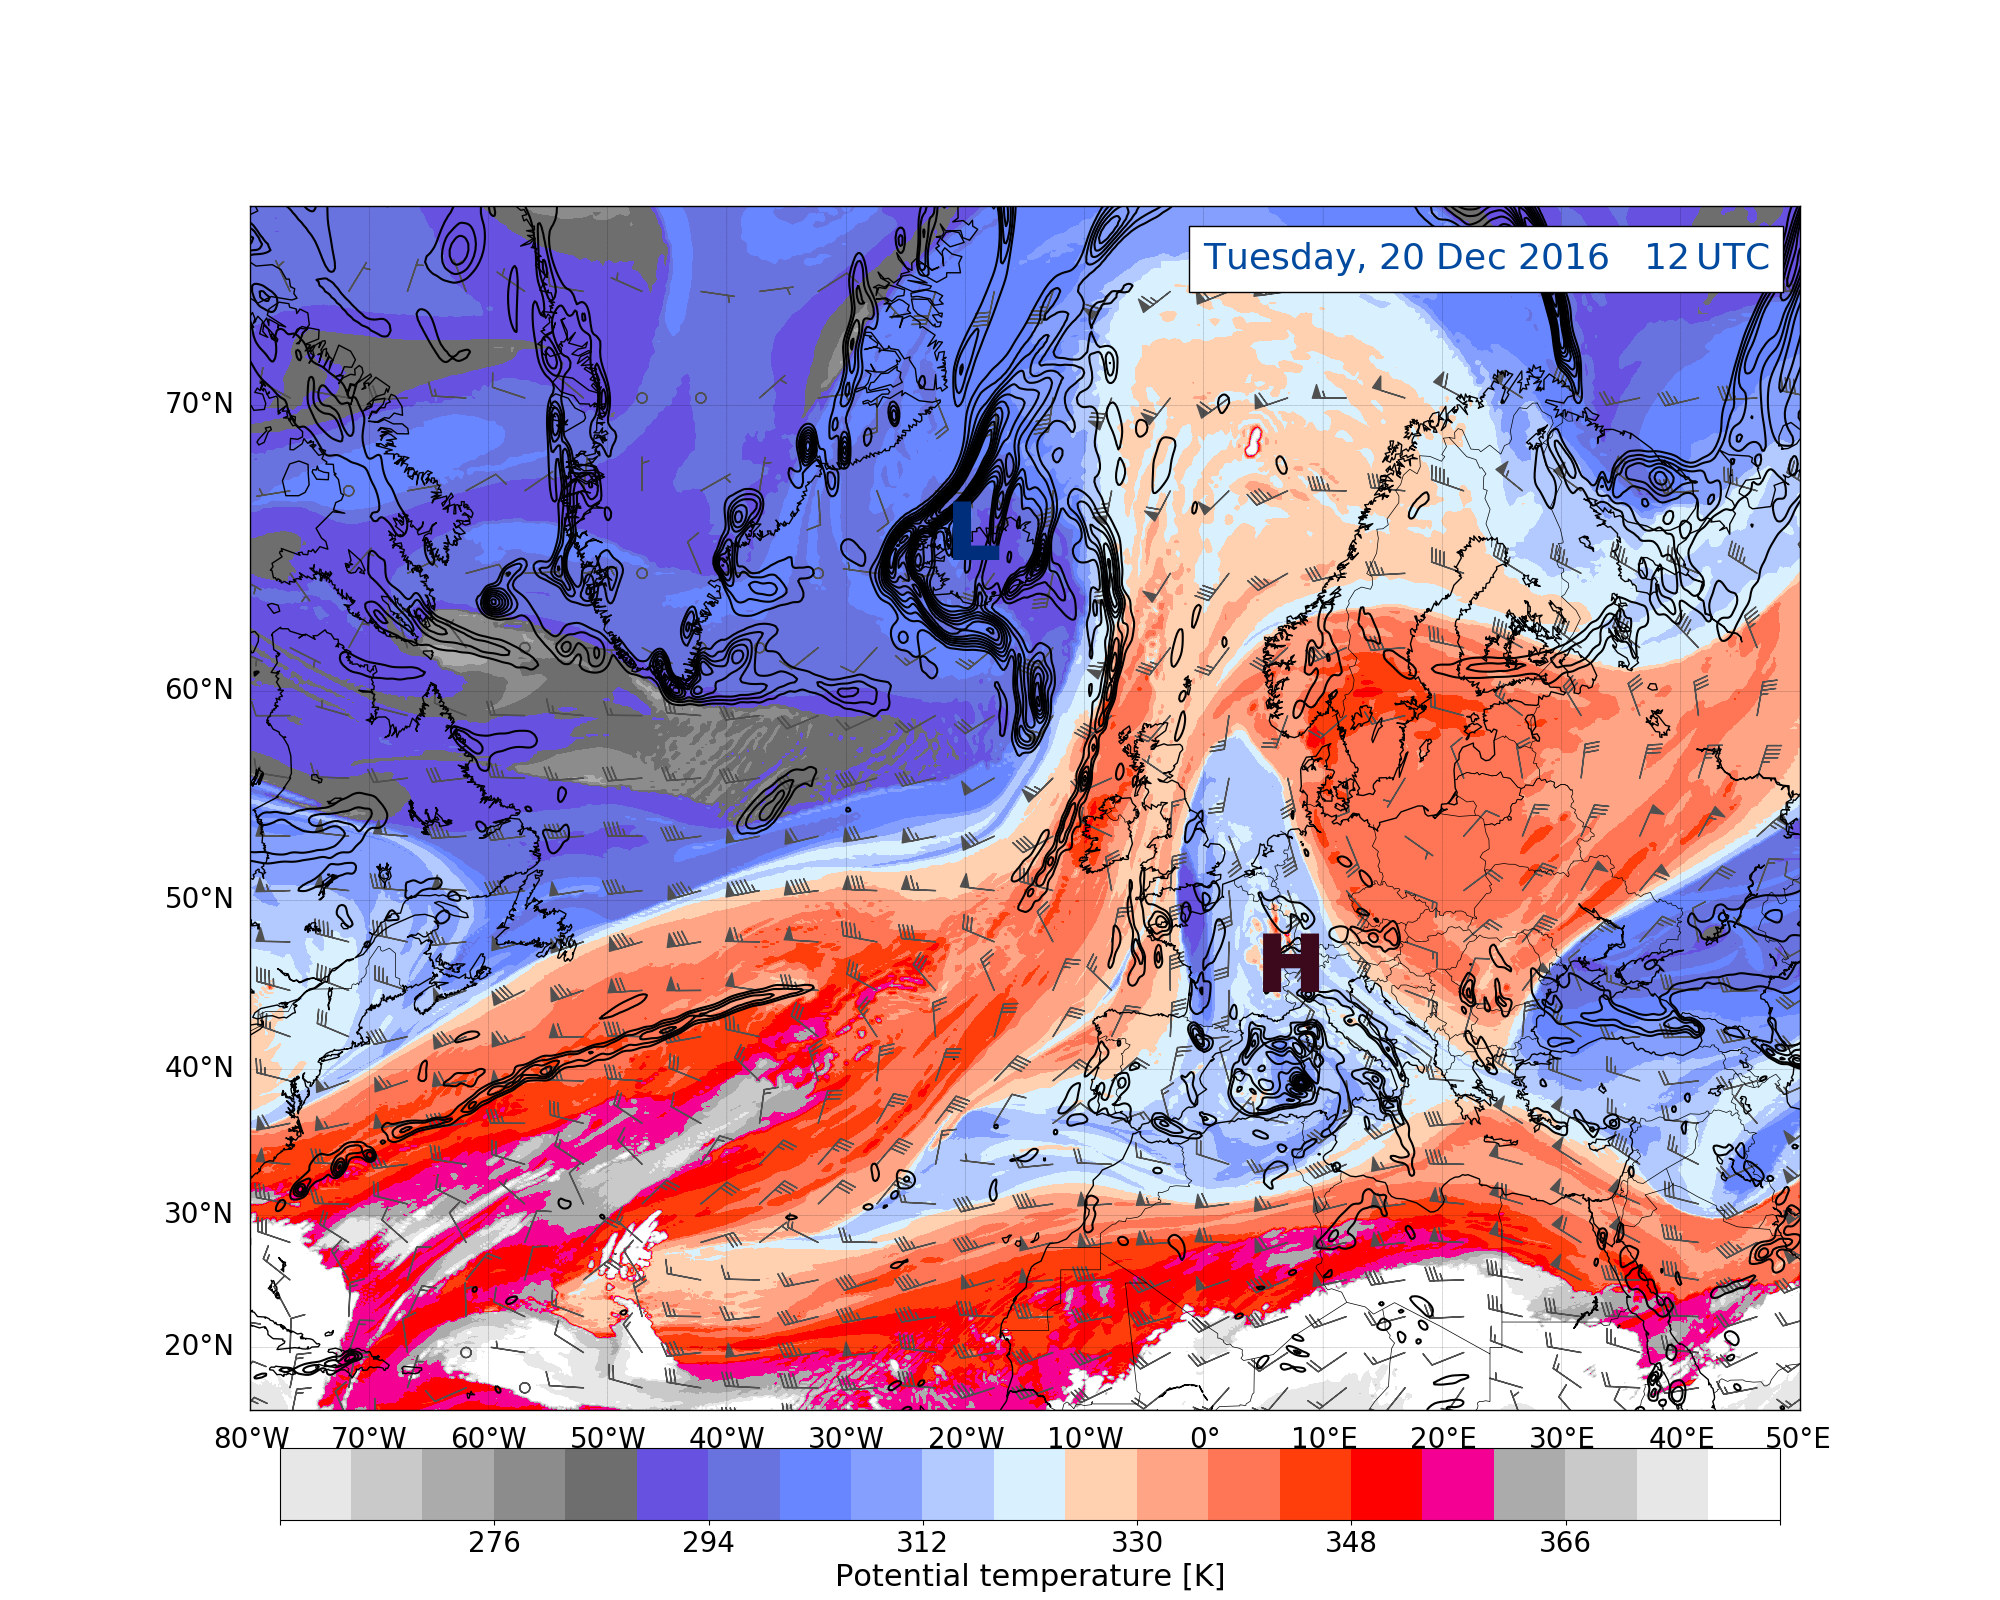
\includegraphics[trim={4.2cm 3.9cm 4.3cm 5.1cm},clip,
		width=\textwidth]{./fig_DynTropo/20161220_12}
		\caption{} \label{fig:DT20}
	\end{subfigure}
	%%%%%% 21/12
	\begin{subfigure}[b]{0.49\textwidth}
		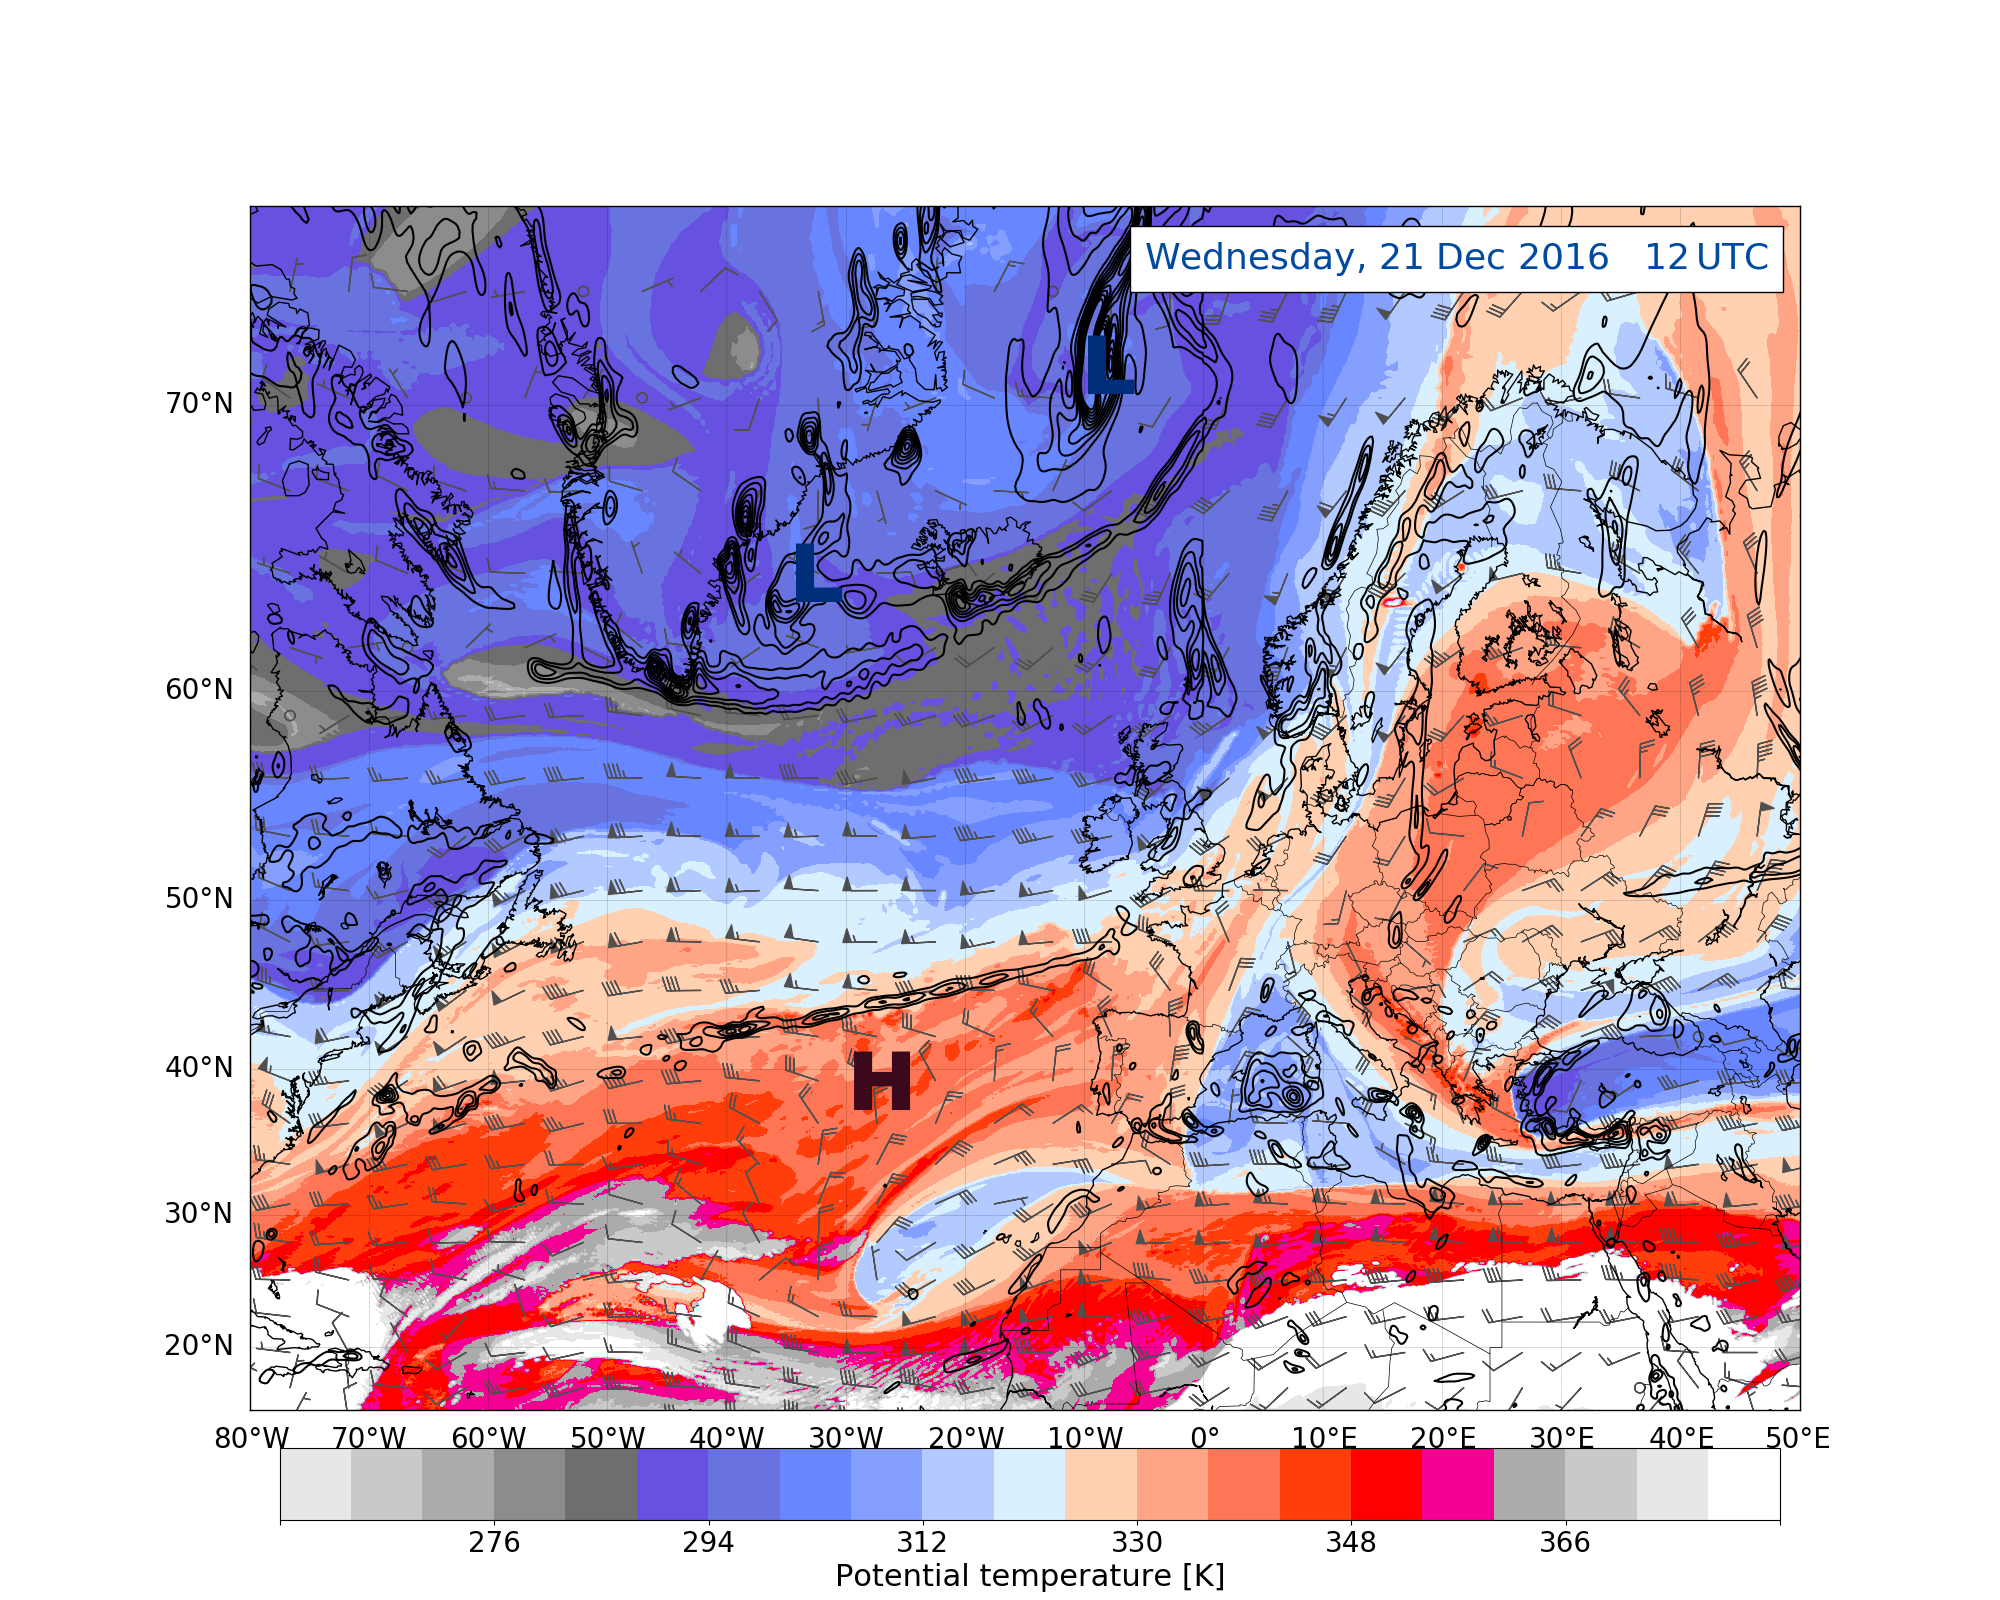
\includegraphics[trim={4.2cm 3.9cm 4.3cm 5.1cm},clip,
		width=\textwidth]{./fig_DynTropo/20161221_12}
		\caption{}\label{fig:DT21}
	\end{subfigure}
	
	%%%%%% 22/12
	\begin{subfigure}[b]{0.49\textwidth}
		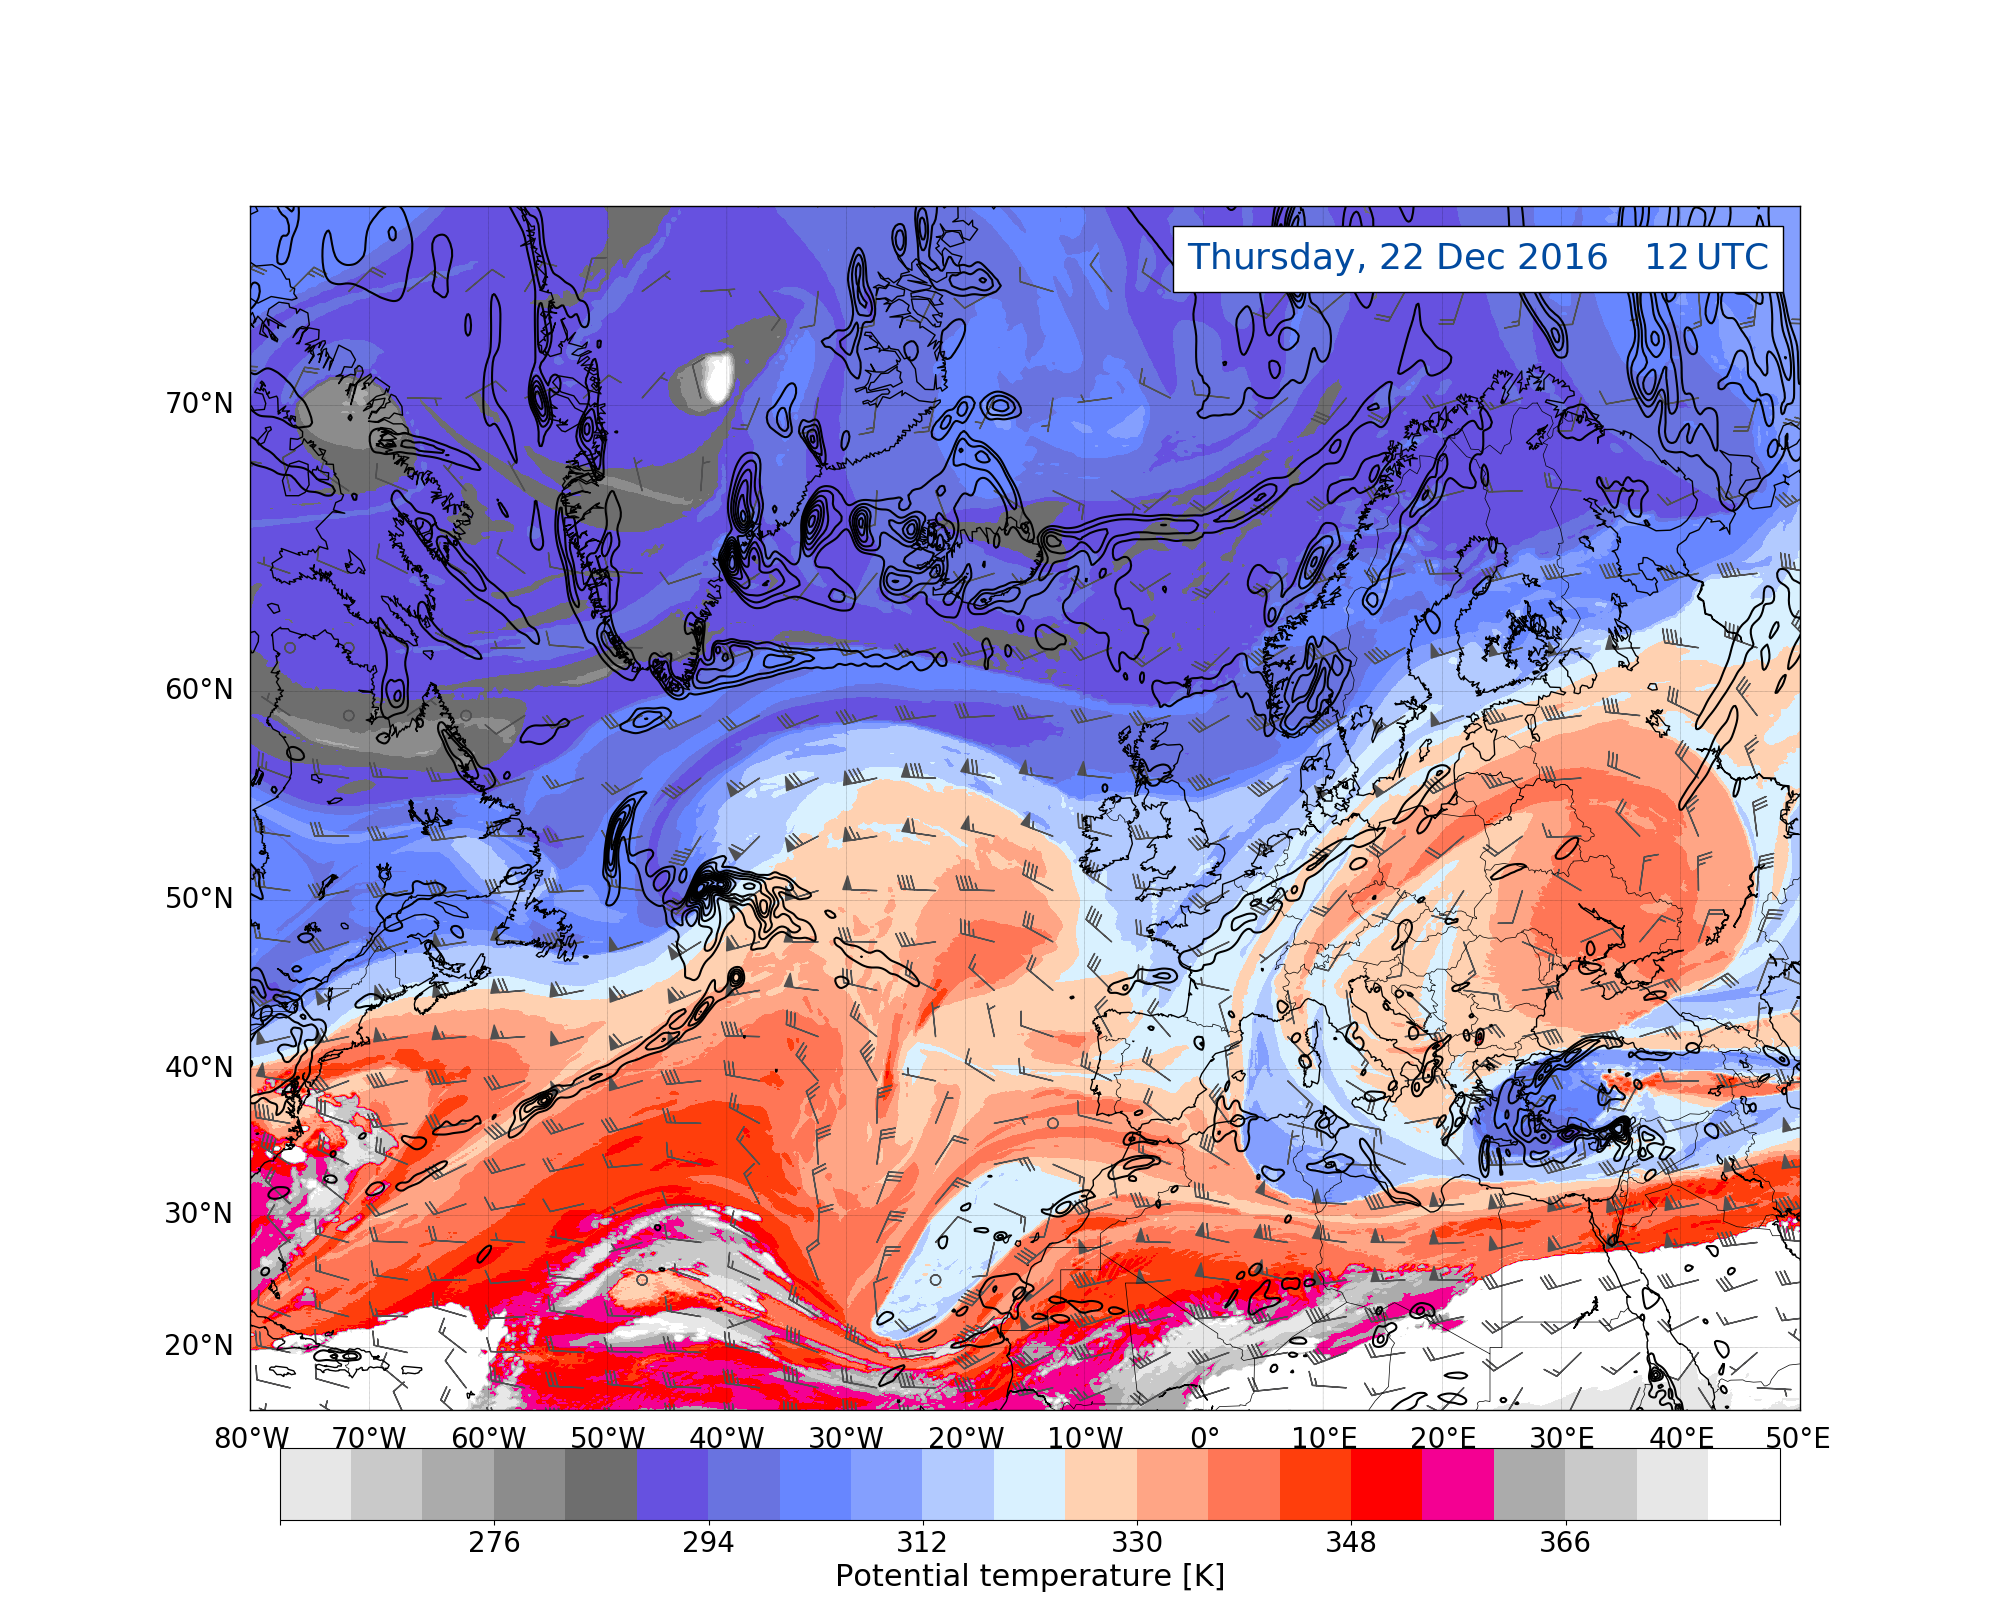
\includegraphics[trim={4.2cm 3.9cm 4.3cm 5.1cm},clip,
		width=\textwidth]{./fig_DynTropo/20161222_12}
		\caption{}\label{fig:DT22}
	\end{subfigure}
	%%%%%% 23/12
	\begin{subfigure}[b]{0.49\textwidth}
		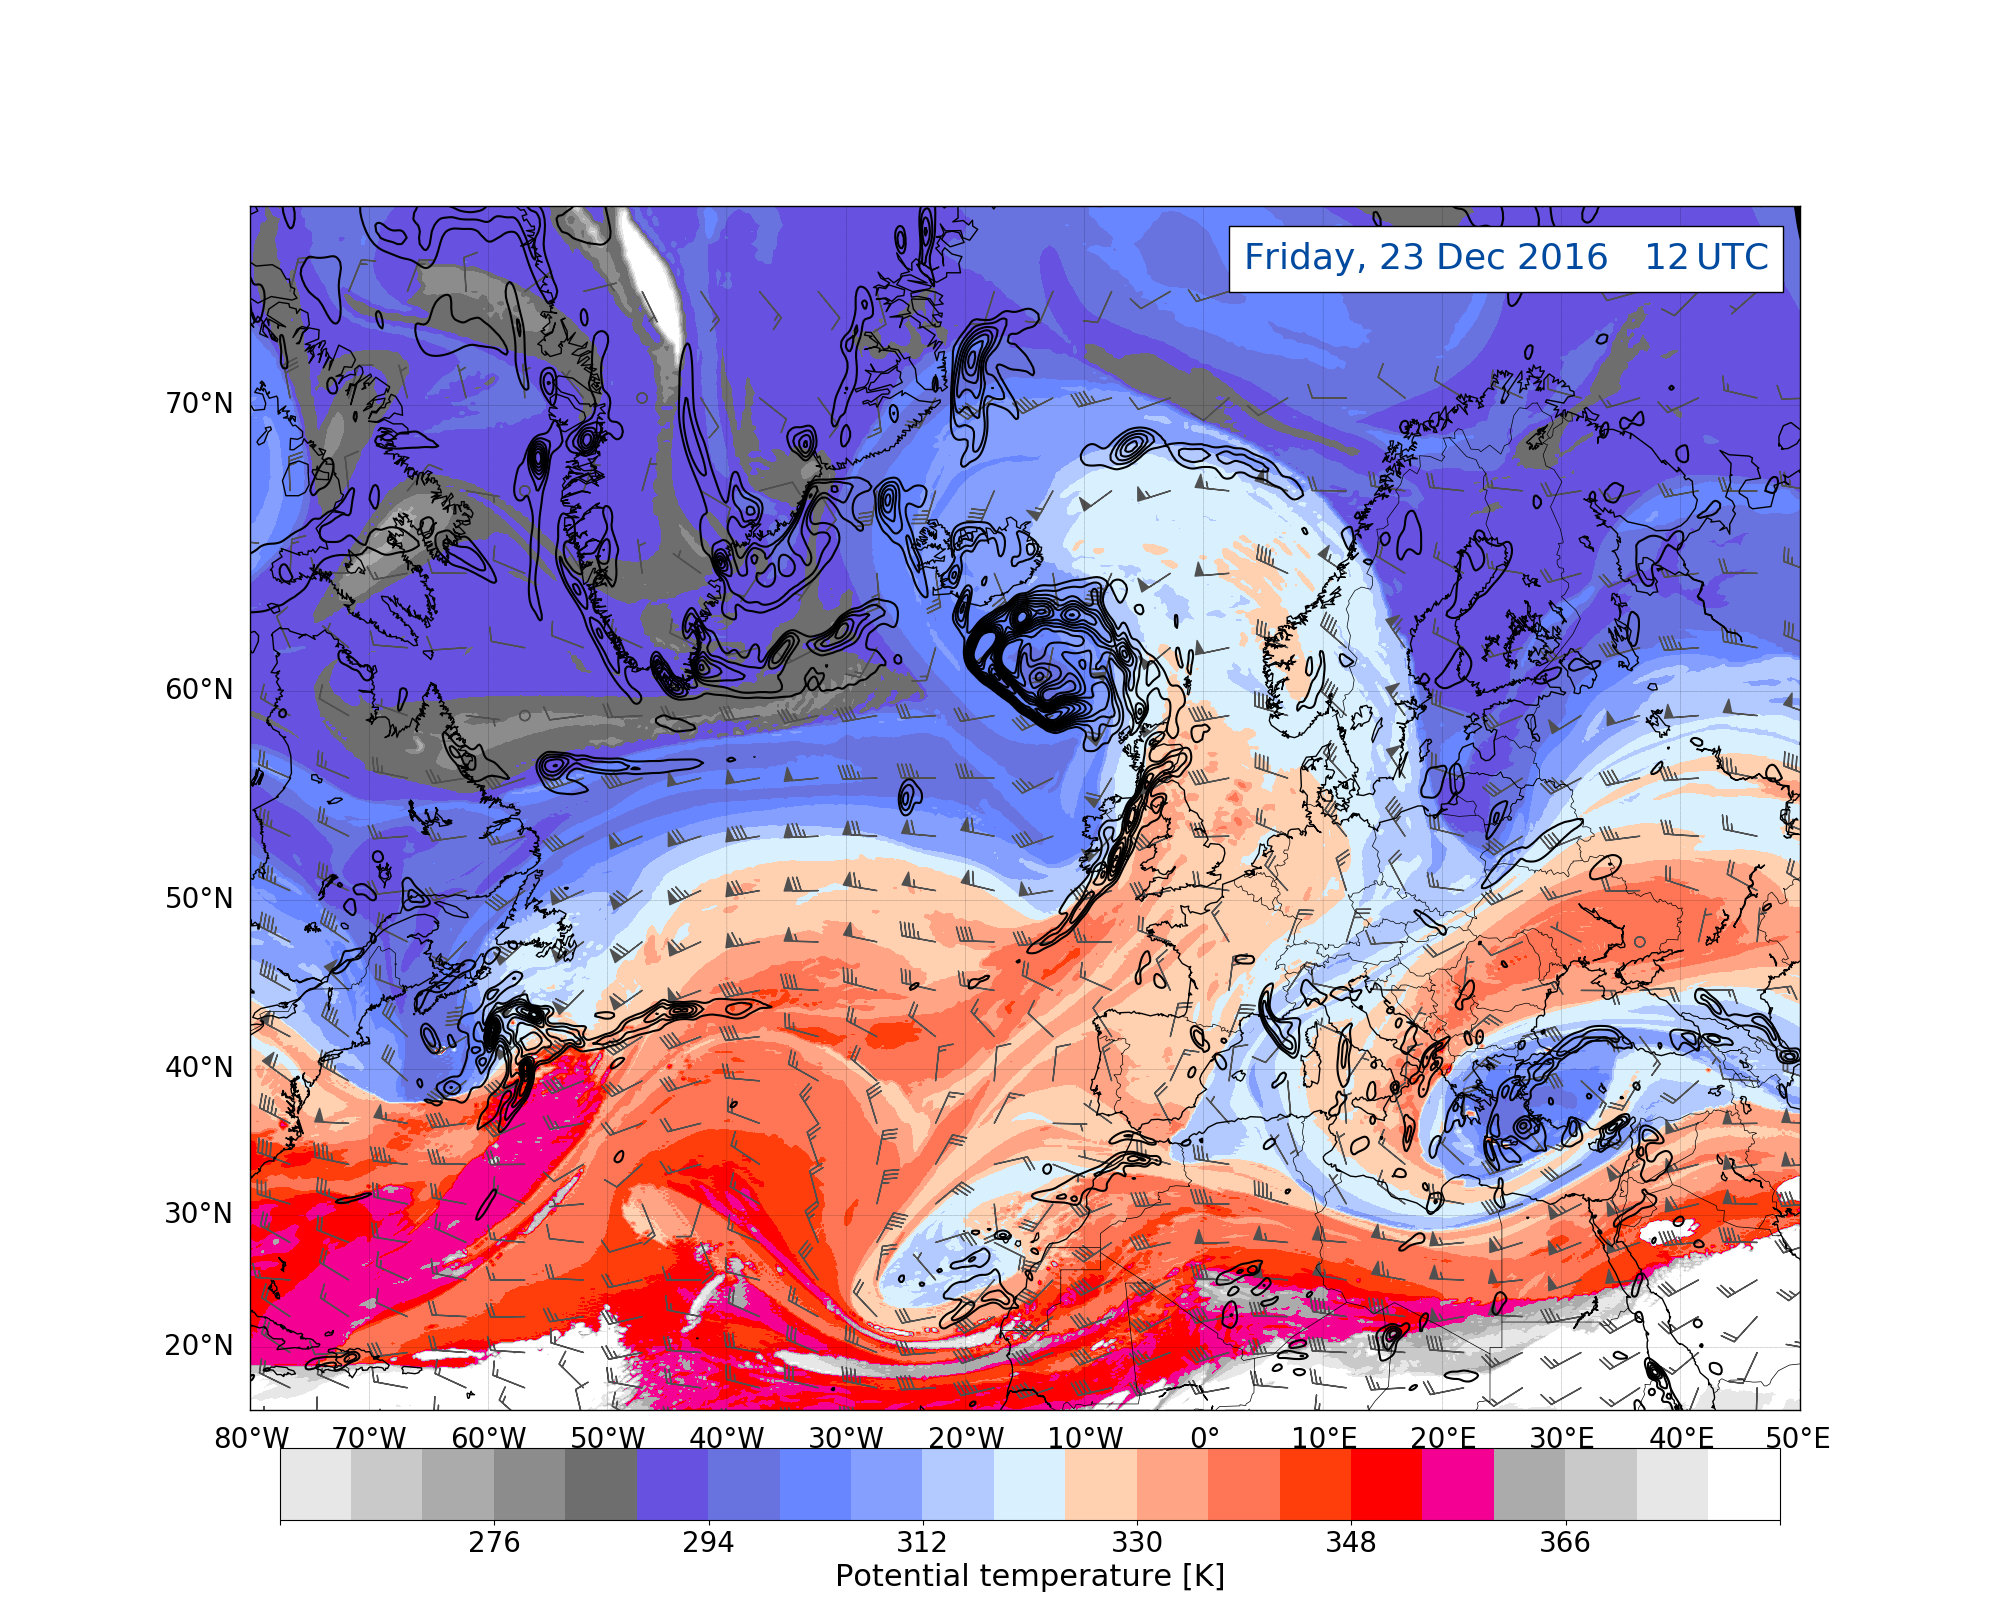
\includegraphics[trim={4.2cm 3.9cm 4.3cm 5.1cm},clip,
		width=\textwidth]{./fig_DynTropo/20161223_12}
		\caption{}\label{fig:DT23}
	\end{subfigure}
	
	%%%%%% label
	\begin{subfigure}[b]{\textwidth}
		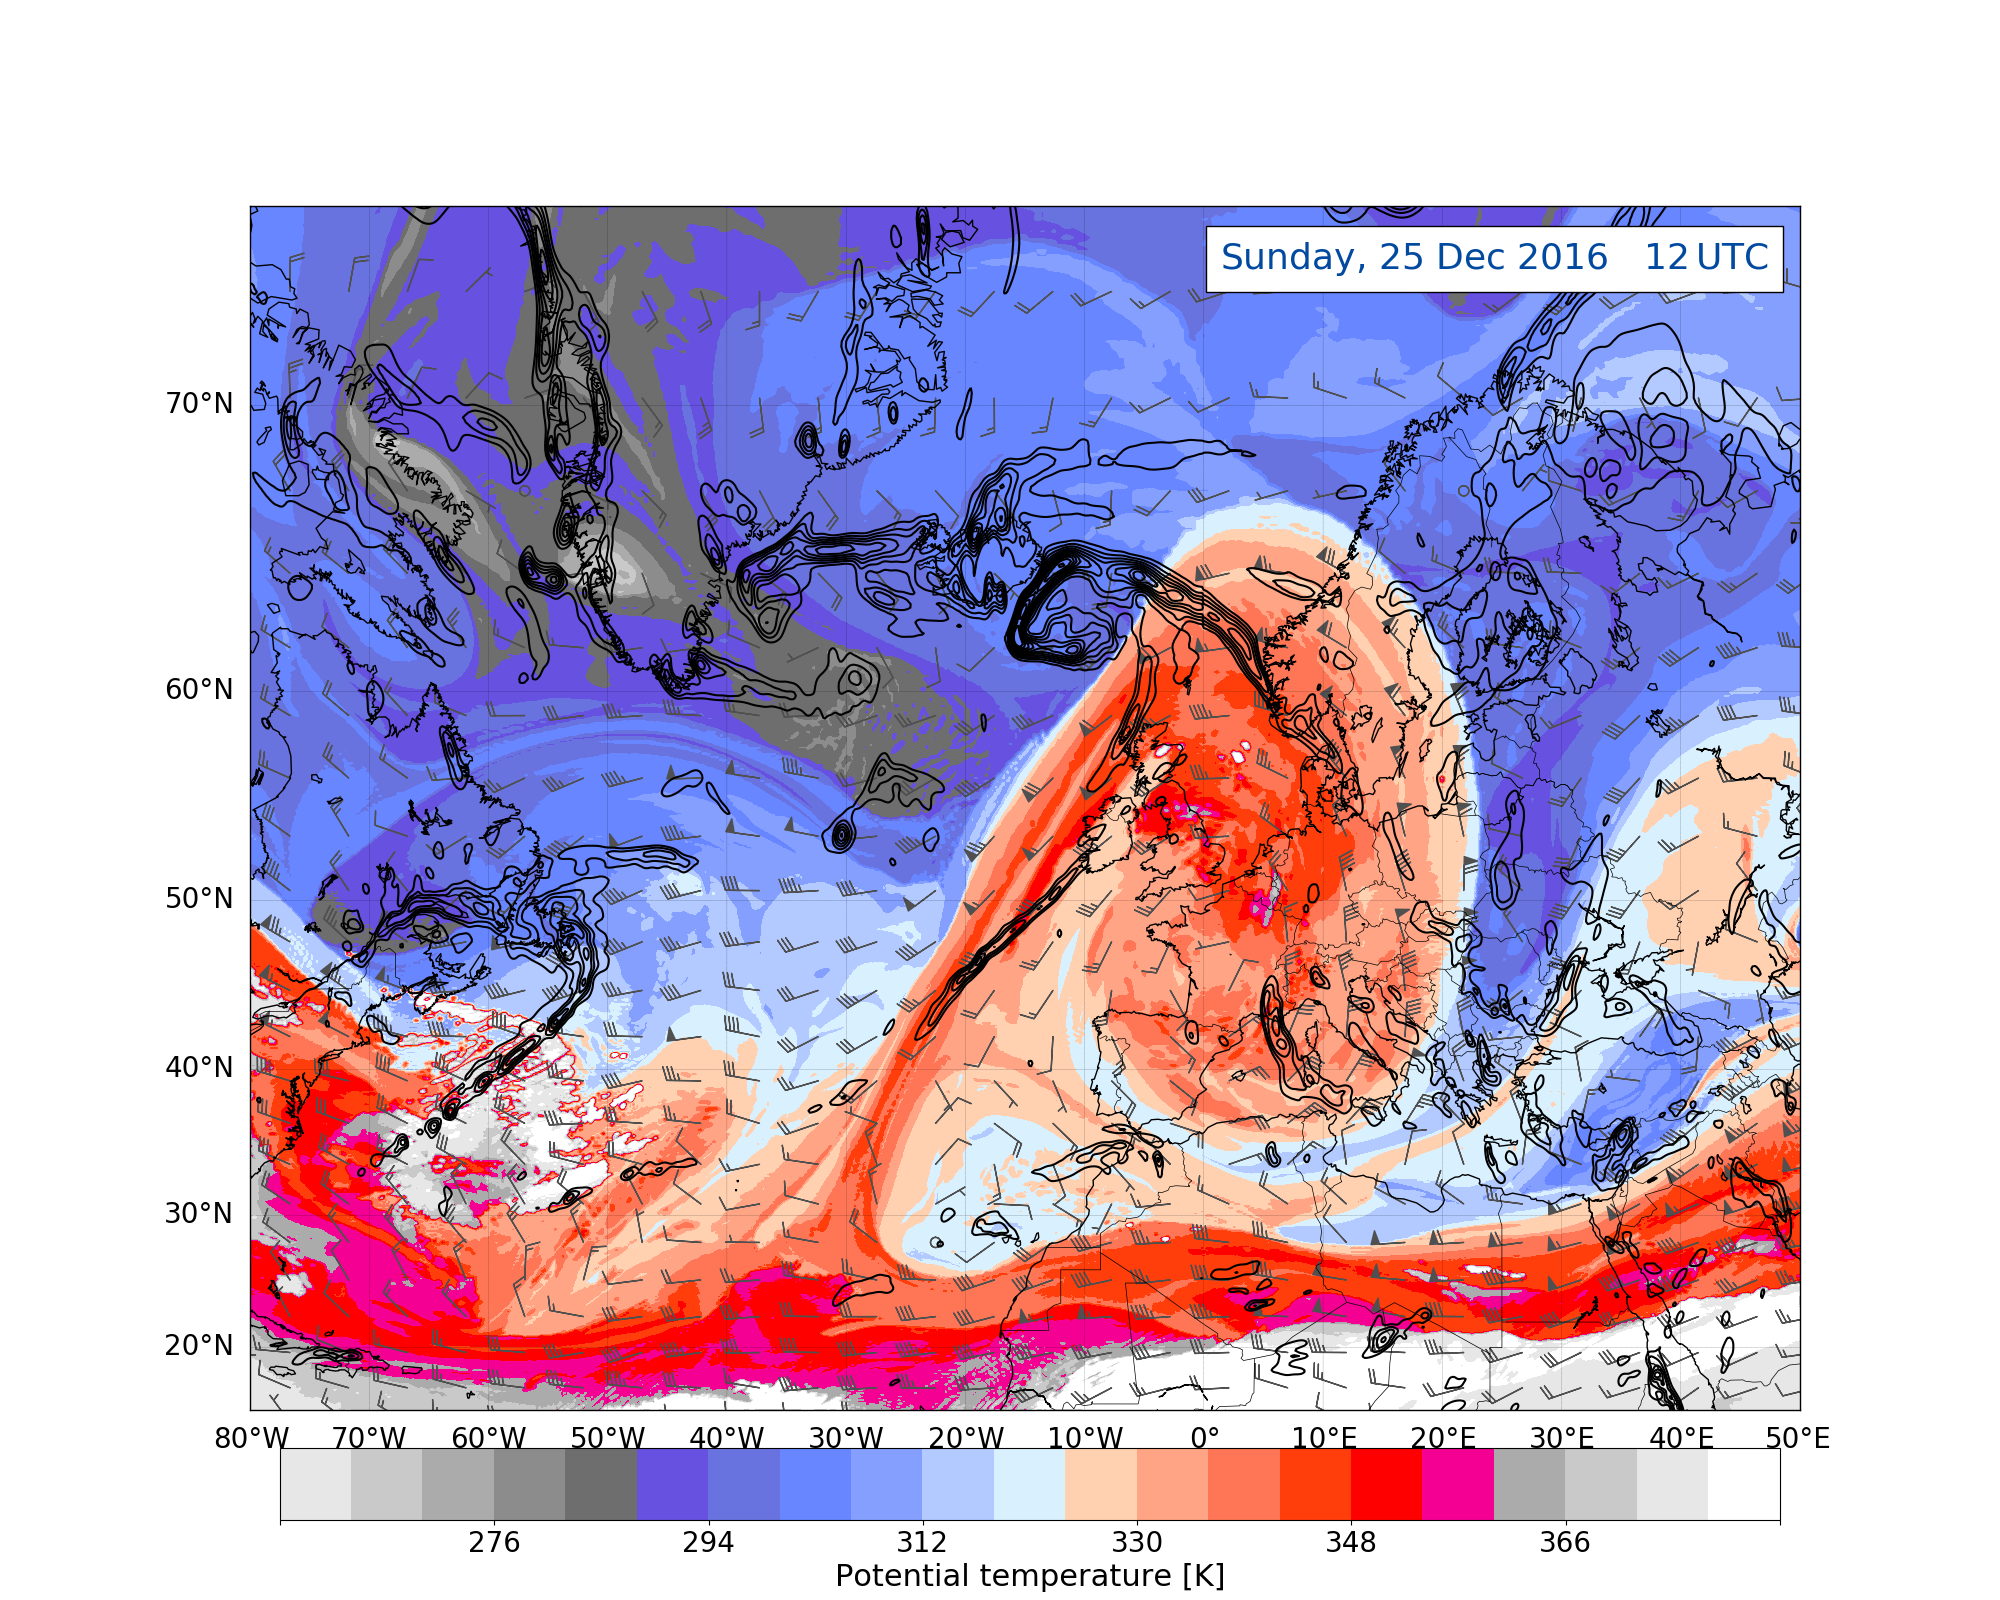
\includegraphics[trim={4.2cm 0cm 4.3cm 36.8cm},clip,
		width=\textwidth]{./fig_DynTropo/20161225_12}
	\end{subfigure}
\end{figure}
%
\begin{figure}\ContinuedFloat
	\centering
	%%%%%% 24/12
	\begin{subfigure}[b]{0.49\textwidth}
		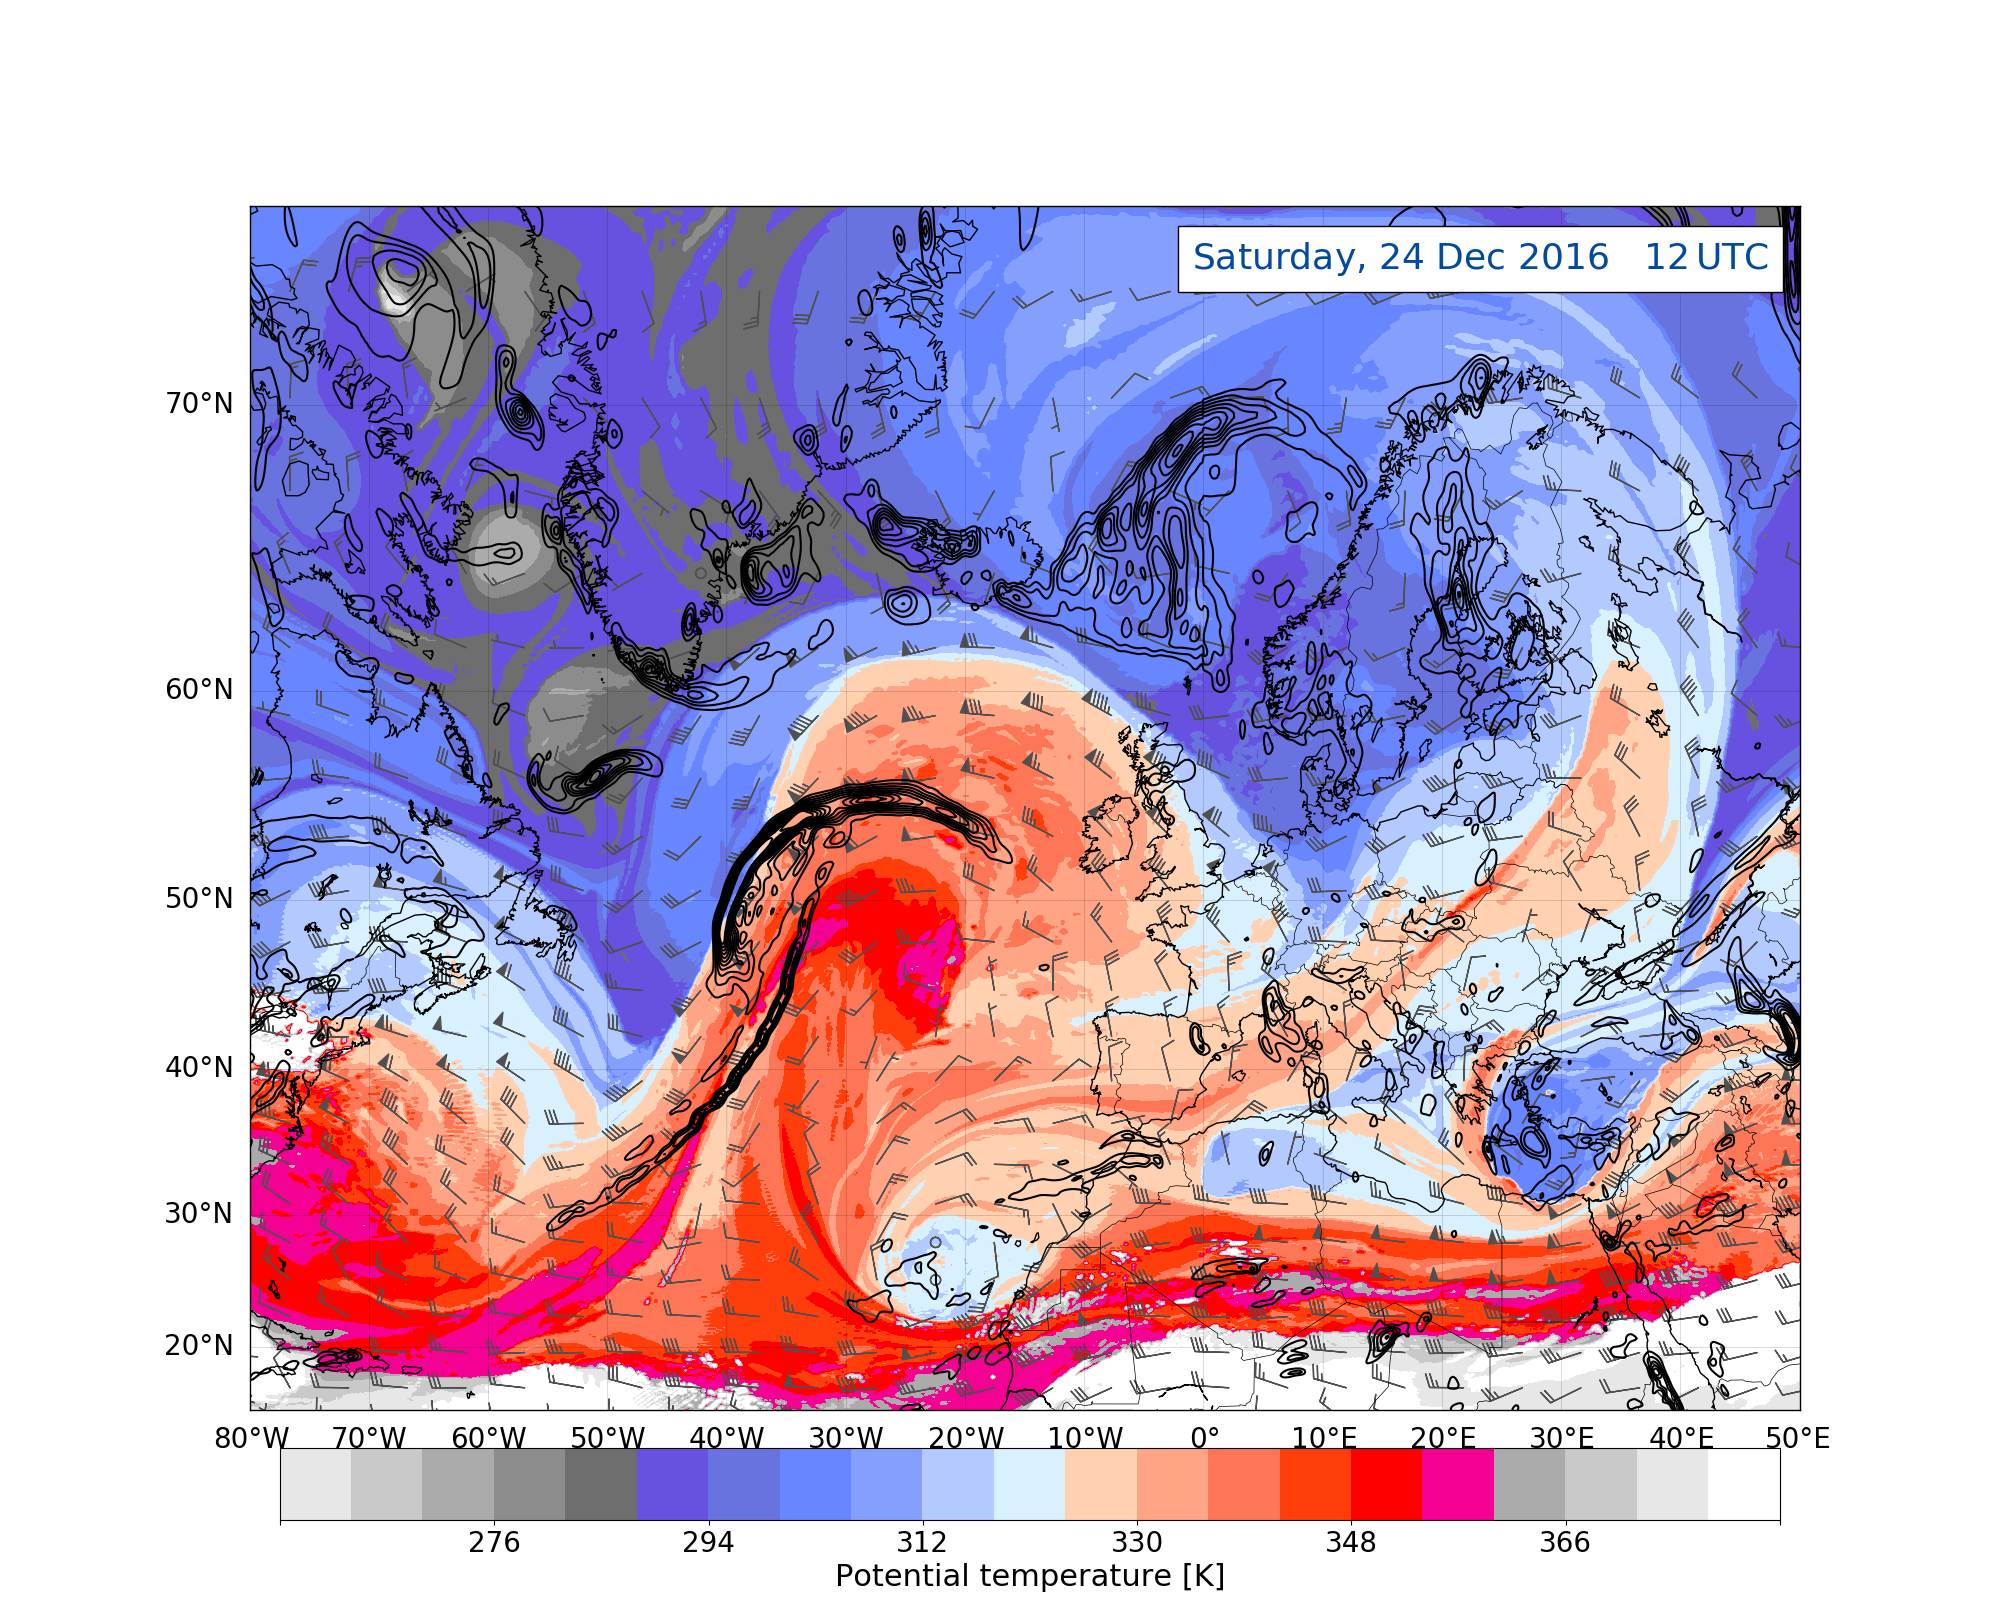
\includegraphics[trim={4.2cm 3.9cm 4.3cm 5.1cm},clip,
		width=\textwidth]{./fig_DynTropo/20161224_12}
		\caption{}\label{fig:DT24}
	\end{subfigure}
	%%%%%% 25/12
	\begin{subfigure}[b]{0.49\textwidth}
		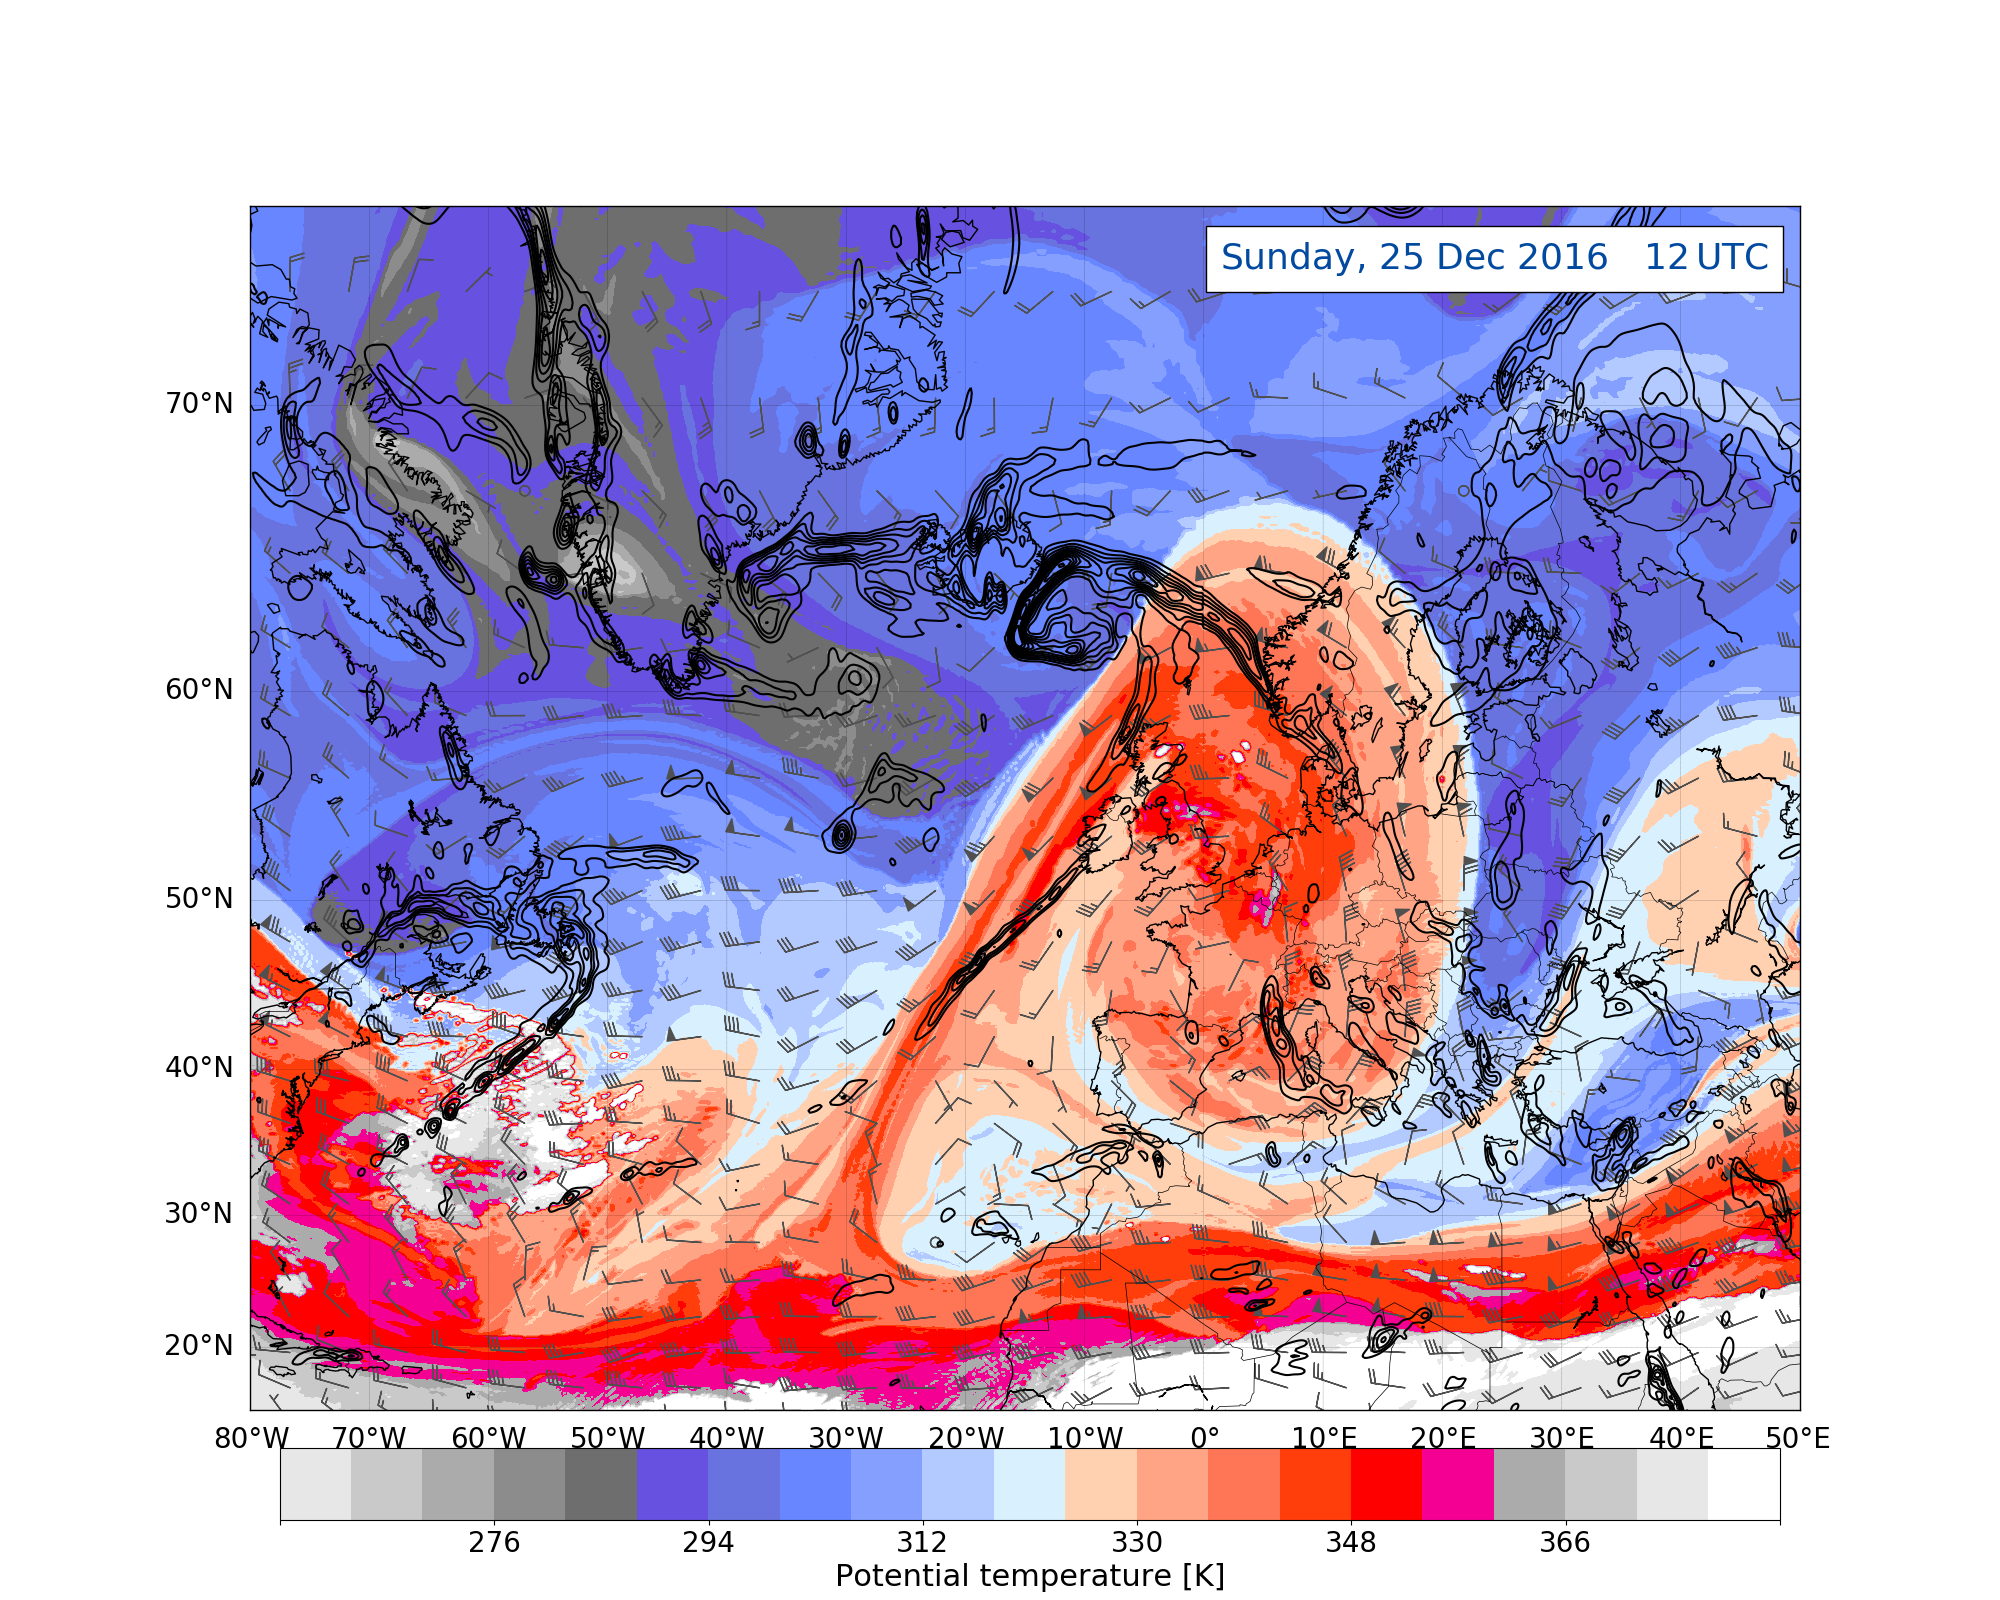
\includegraphics[trim={4.2cm 3.9cm 4.3cm 5.1cm},clip,
		width=\textwidth]{./fig_DynTropo/20161225_12}
		\caption{}\label{fig:DT25}
	\end{subfigure}    
	%%%%%% 26/12
	\begin{subfigure}[b]{0.49\textwidth}
		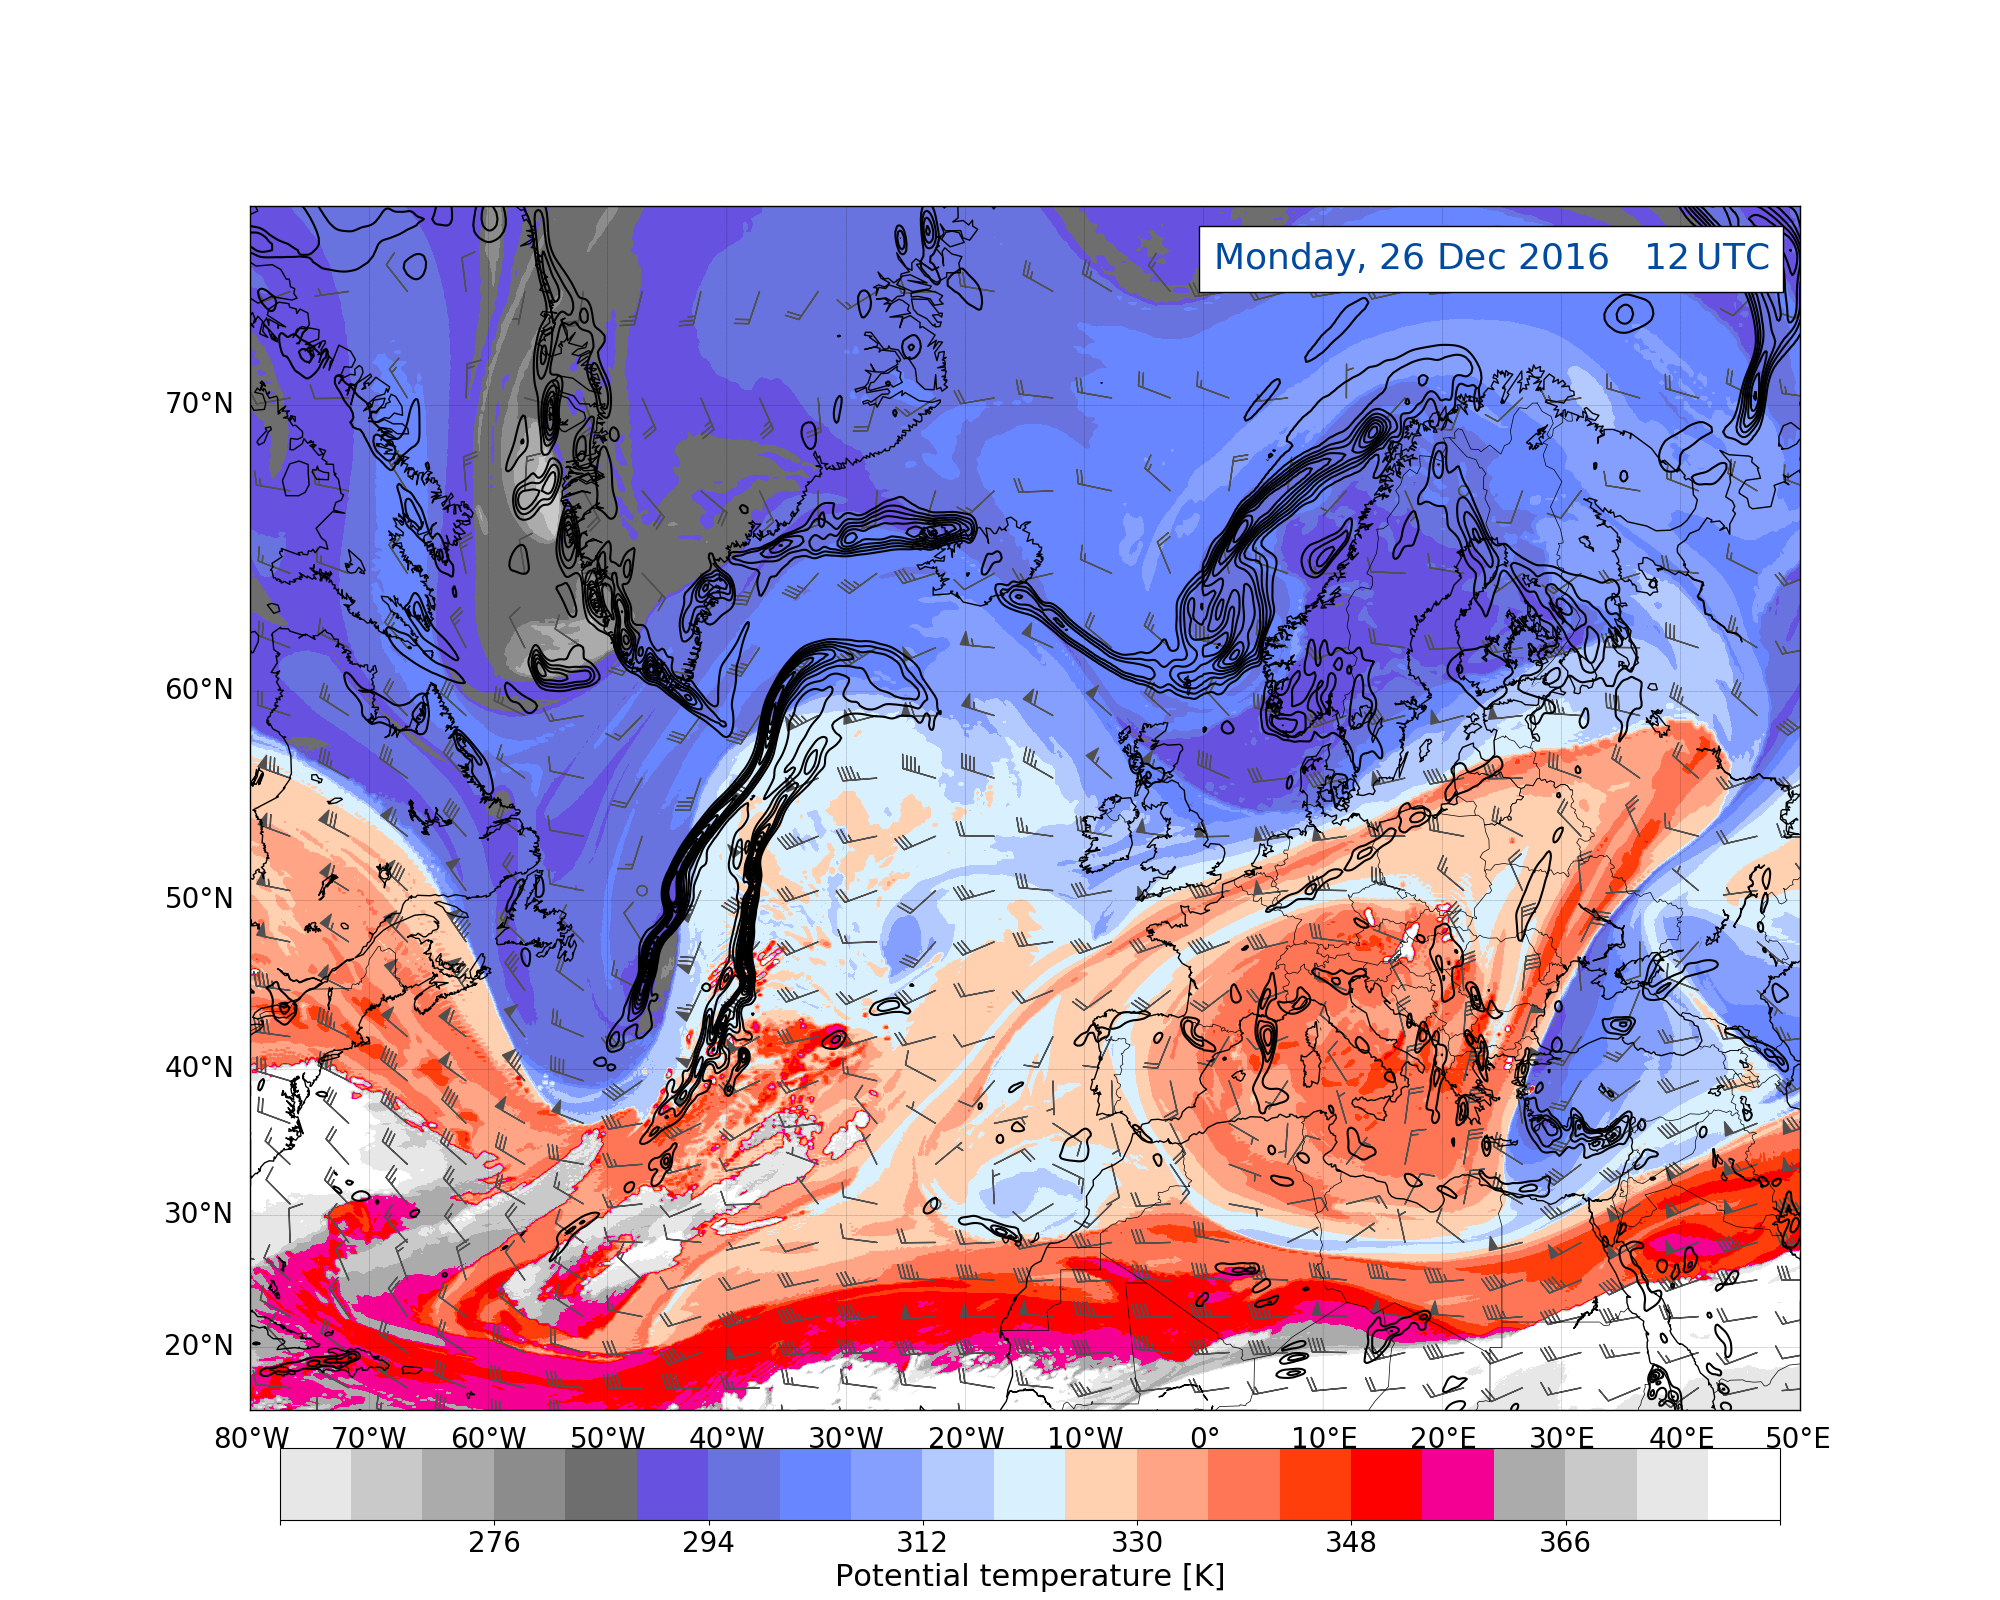
\includegraphics[trim={4.2cm 3.9cm 4.3cm 5.1cm},clip,
		width=\textwidth]{./fig_DynTropo/20161226_12}
		\caption{}\label{fig:DT26}
	\end{subfigure}
	%%%%%% 27/12
	\begin{subfigure}[b]{0.49\textwidth}
		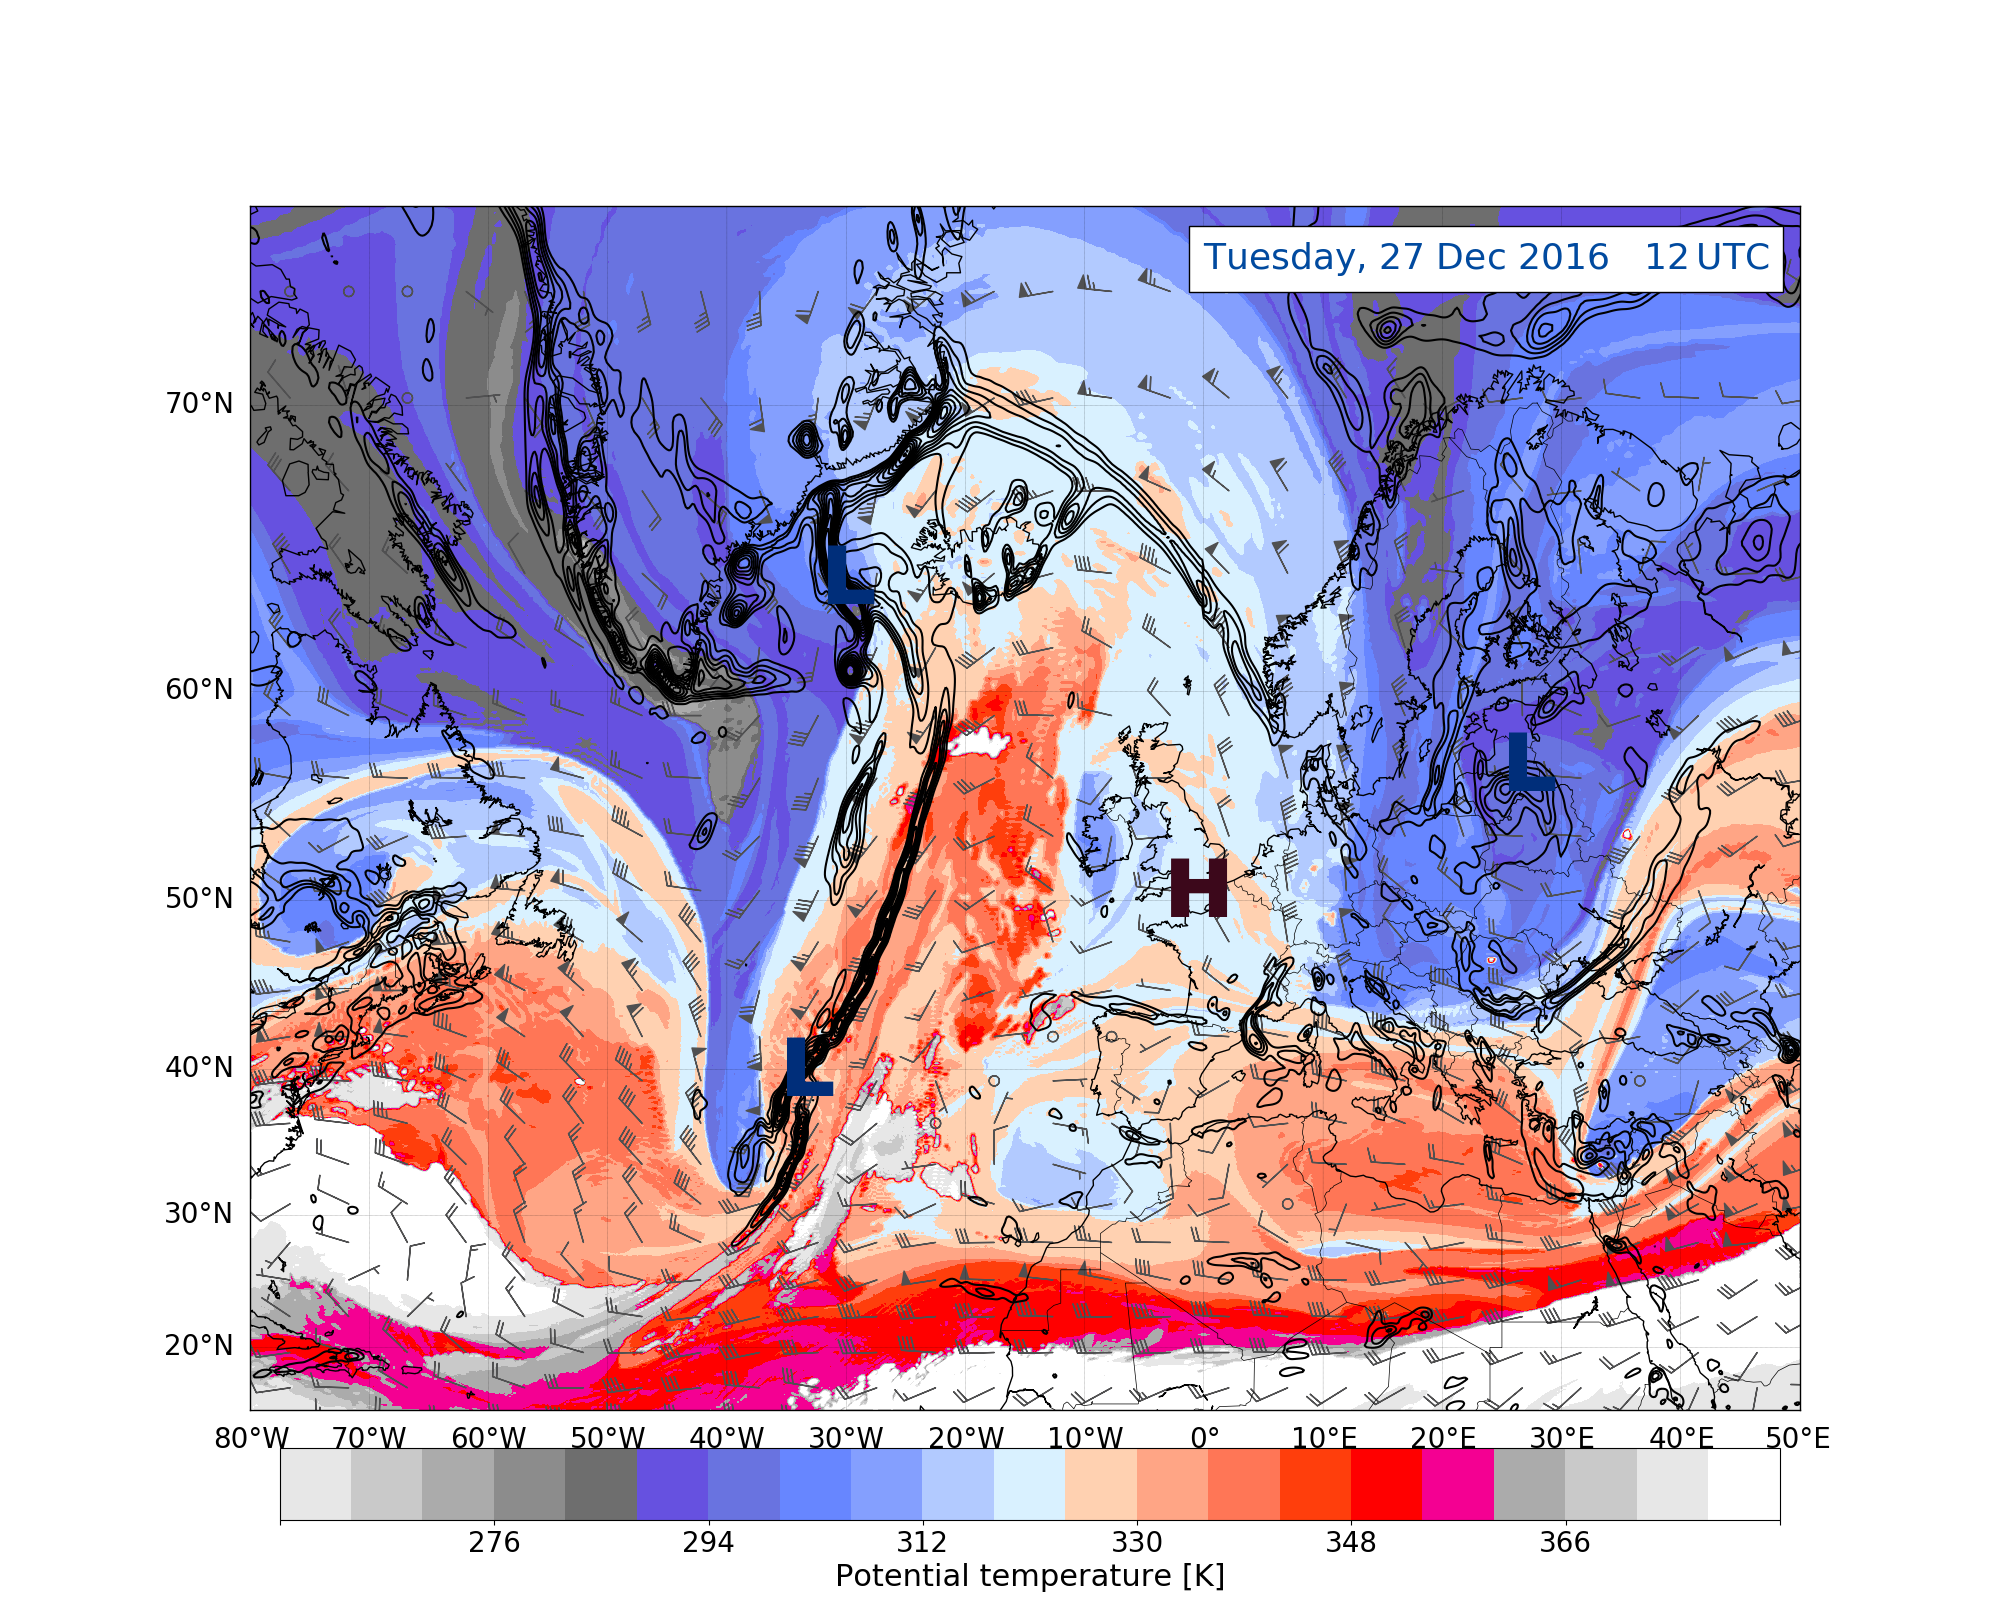
\includegraphics[trim={4.2cm 3.9cm 4.3cm 5.1cm},clip,
		width=\textwidth]{./fig_DynTropo/20161227_12}
		\caption{}\label{fig:DT27}
	\end{subfigure}   
	%%%%%% label
	\begin{subfigure}[b]{\textwidth}
		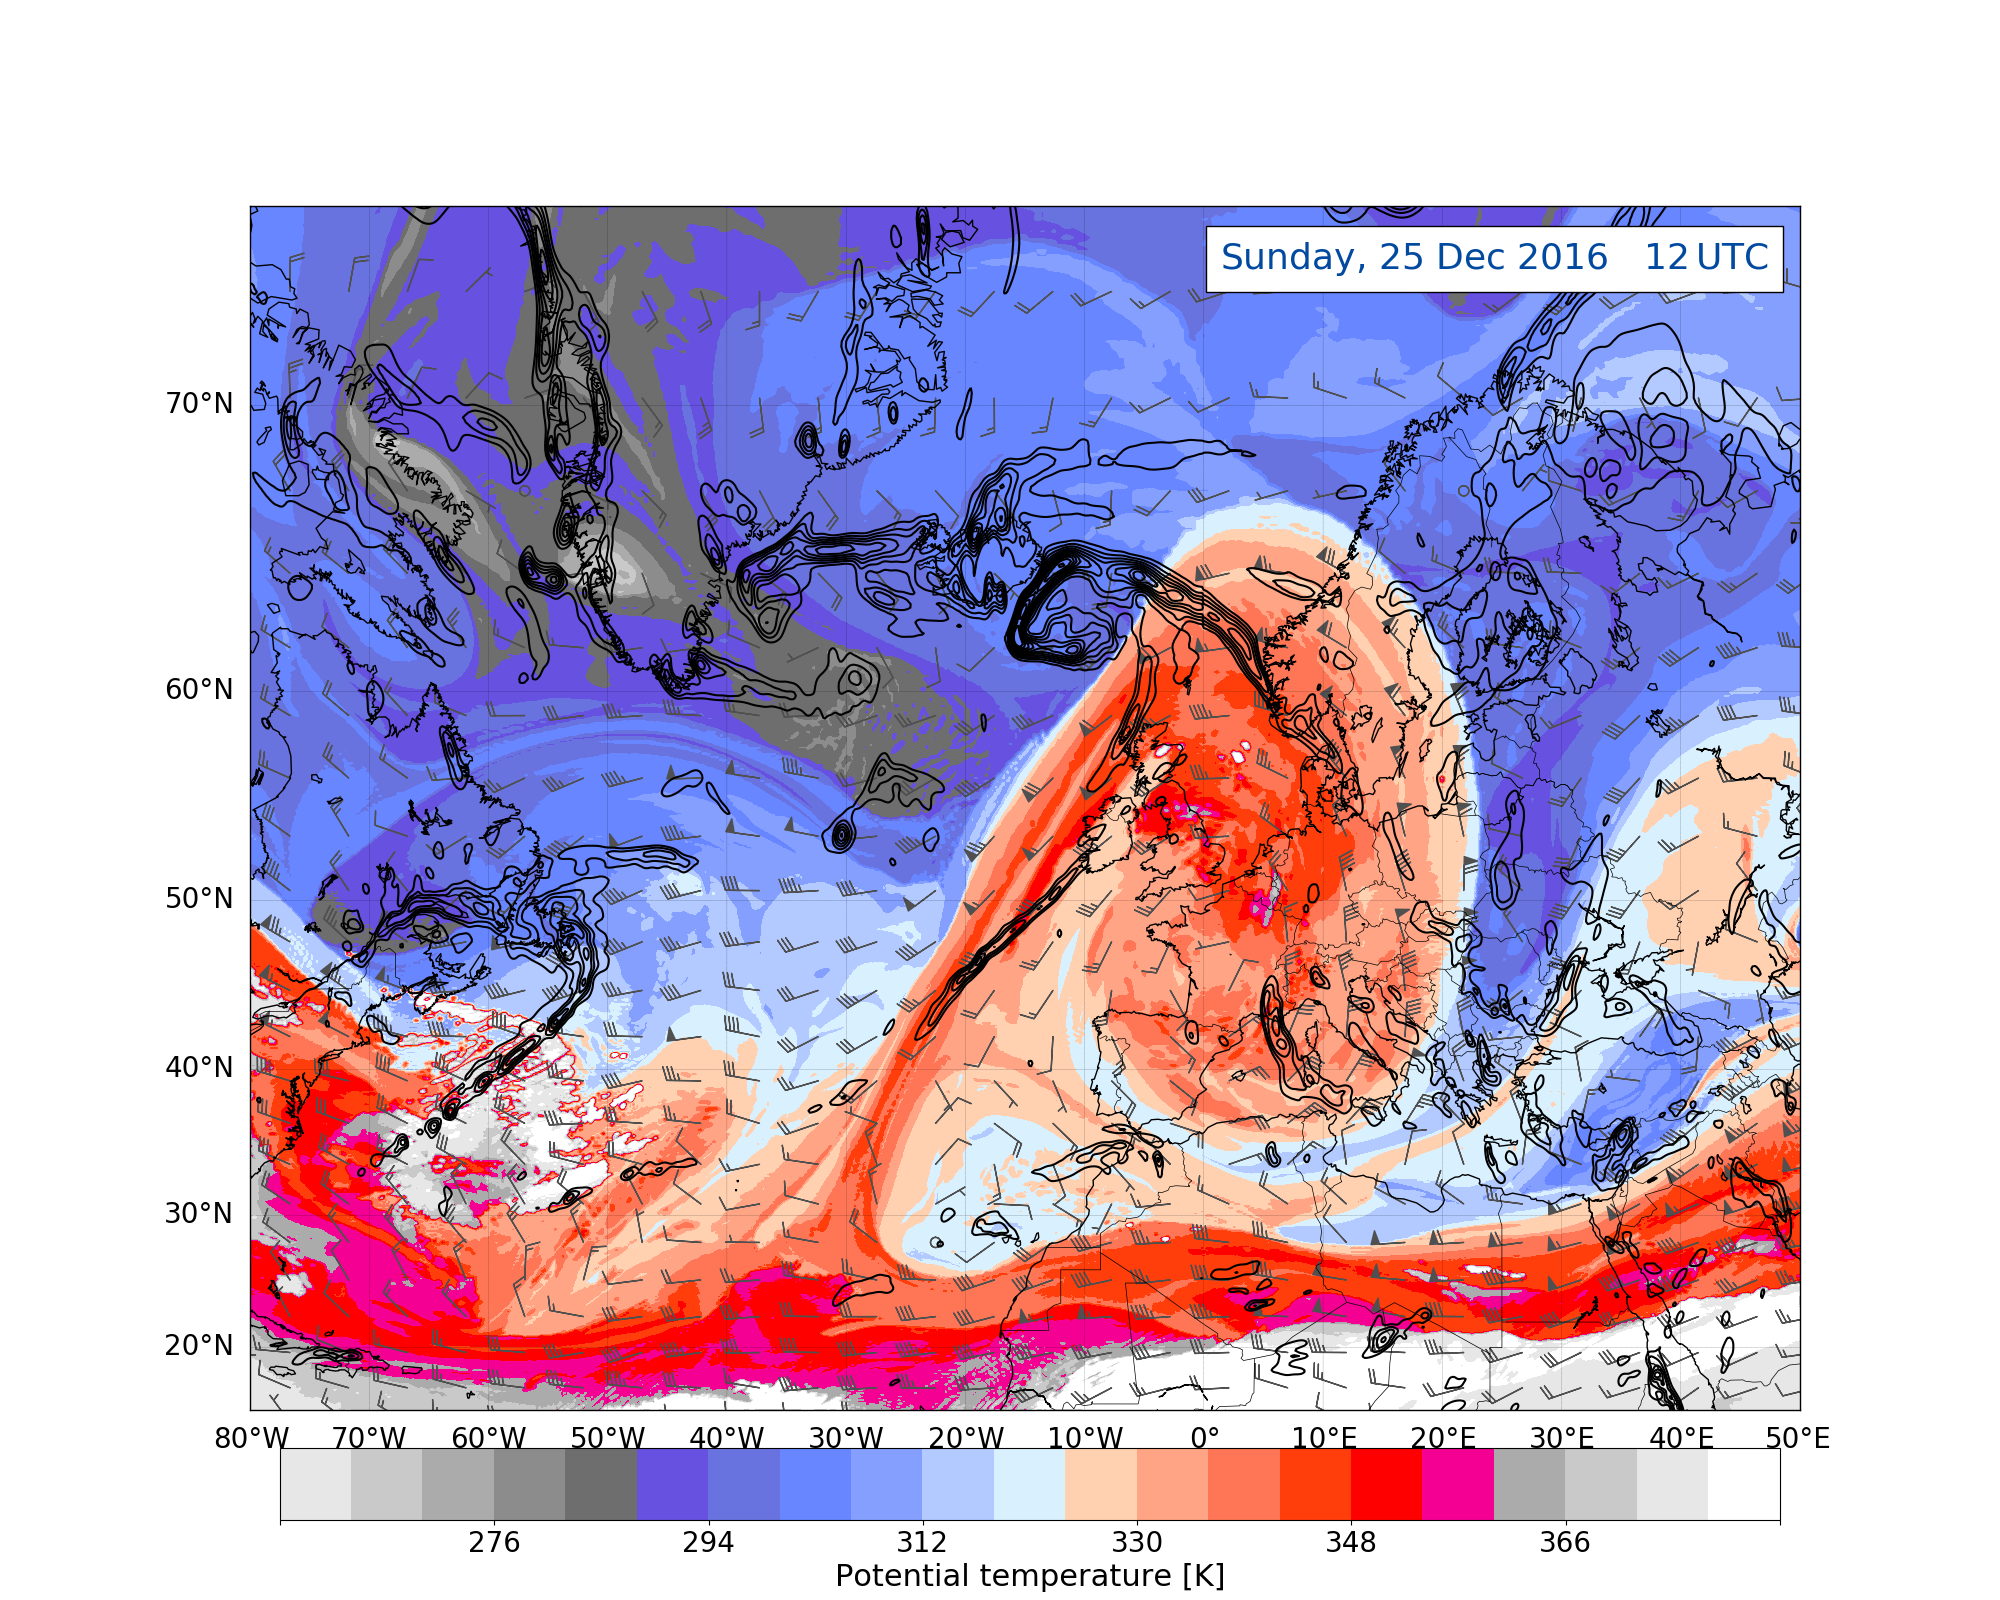
\includegraphics[trim={4.2cm 0cm 4.3cm 36.8cm},clip,
		width=\textwidth]{./fig_DynTropo/20161225_12}
	\end{subfigure}
	\caption{Dynamic tropopause analysis map, data from ECMWF at \SI{2}{PVU}. During \SIrange{20}{27}{\dec}. Potential temperature [K] at the \SI{2}{PVU} surface, shaded according to the colour bar. Total wind, barbs [\SI{}{\mPs}], and \SI{925}-\SI{850}{\hPa} layer-averaged surface relative vorticity (black contours, every \SI{.5e-4}{\per\second}).  }\label{fig:DynTropo}
\end{figure}